\section{Powers, Polynomials, and Rational Functions} \label{S.0.6.PowersPolysRationals}


\vspace*{-14 pt}
\framebox{\hspace*{3 pt}
\parbox{6.25 in}
{\begin{goals}
	\item What are power, polynomial, and rational functions?
	\item How can be build polynomial functions from data?
	\item What microscopic/macroscopic behavior can we expect from polynomial and rational functions?
 \end{goals}} 
\hspace*{3 pt}}


% \begin{web}
% \item \href{https://www.khanacademy.org/math/algebra2/polynomial_and_rational}{Khan
%     Playlist: Polynomial and rational functions}
% \item
%     \href{https://www.khanacademy.org/math/algebra2/polynomial_and_rational/rational_funcs_tutorial/v/adding-and-subtracting-rational-expressions}{Khan
%     Playlist: Rational functions}
% \end{web}

\nin \hrulefill


\subsection*{Introduction}

Polynomial functions play an important role in mathematics.  They are generally simple to compute (requiring only computations that can be done by hand) and can be used to model many real-world phenomena.  In fact, scientists and mathematicians frequently simplify complex mathematical models by substituting a polynomial model that is "close enough" for their purposes.

In this section, we will study the graphs of select polynomial and rational functions to identify their important features.  The goal of this section is to build a mathematical intuition about how a small class of 'convenient' functions behave so that later we can see how calculus can be used to determine the behavior of arbitrary functions.

\begin{pa} \label{PA:0.6}
    
Figure \ref{fig:0.6.PA} shows the graphs of two different functions.  Suppose that you were to graph a line anywhere along each of the two graphs.

\begin{enumerate}
	\item Is it possible to draw a line that does not intersect the graph of $f$? $g$?
	\item Is it possible to draw a line that intersects the graph of $f$ an even number of times?
	\item Is it possible to draw a line that intersects the graph of $g$ an odd number of times?
	\item What is the fewest number of intersections that your line could have with the graph of $f$? with $g$?
	\item What is the largest number of intersections that your line could have with the graph of $f$? with $g$?
	\item How many times does the graph of $f$ change directions? How many times does the graph of $g$ change directions?
\end{enumerate}

\begin{figure}[ht!]

	\begin{center}
		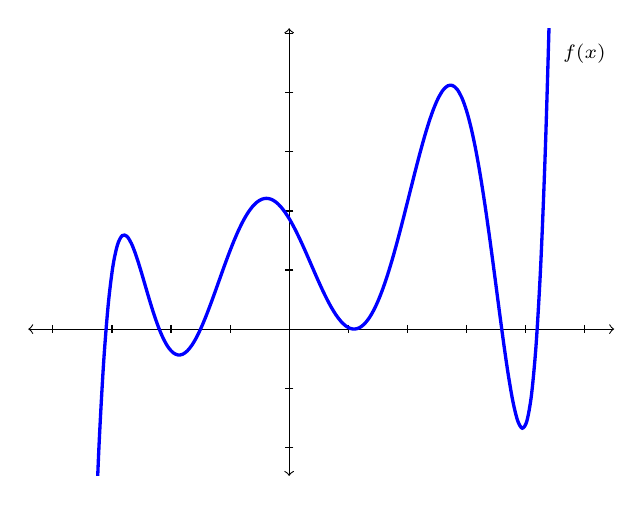
\begin{tikzpicture}[scale=0.75]
			[line cap=round,line join=round,>=triangle 45,x=1.0cm,y=1.0cm] 
			\draw[<->,color=black] (-4.418087504107611,0.0) -- (5.504275777242757,0.0); \foreach \x in {-4.0,-3.0,-2.0,-1.0,1.0,2.0,3.0,4.0,5.0} 
			\draw[shift={(\x,0)},color=black] (0pt,2pt) -- (0pt,-2pt); 
			\draw[<->] (0.0,-2.486833997057605) -- (0.0,5.09438316608086); \foreach \y in {-2.0,-1.0,1.0,2.0,3.0,4.0,5.0} 
			\draw[shift={(0,\y)},color=black] (2pt,0pt) -- (-2pt,0pt); 
			\clip(-4.418087504107611,-2.486833997057605) rectangle (5.504275777242757,5.09438316608086); 
			\draw[color=blue, very thick,smooth,samples=100,domain=-3.3:4.5]
			plot(\x,{((\x)-1.1)^(2.0)*((\x)-3.6)*((\x)+1.5)*((\x)-4.2)*((\x)+2.2)*((\x)+3.1)/100.0});
			\begin{scriptsize}
				\draw[color=black] (5,4.671245463952202) node {$f(x)$};
			\end{scriptsize}
		\end{tikzpicture}
		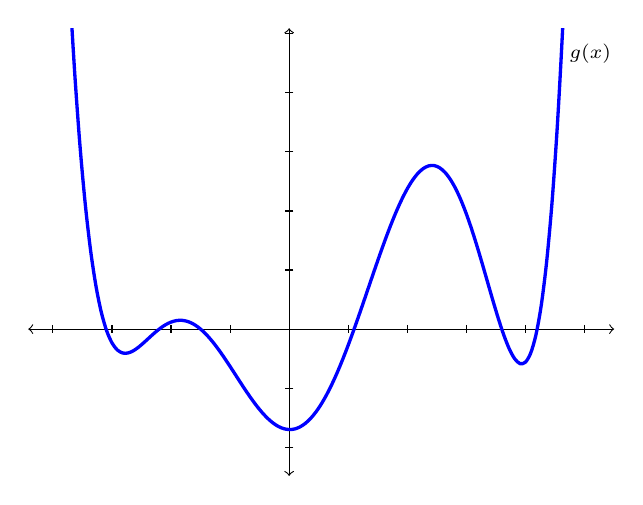
\begin{tikzpicture}[scale=0.75]
			[line cap=round,line join=round,>=triangle 45,x=1.0cm,y=1.0cm] 
			\draw[<->,color=black] (-4.418087504107611,0.0) -- (5.504275777242757,0.0); \foreach \x in {-4.0,-3.0,-2.0,-1.0,1.0,2.0,3.0,4.0,5.0} 
			\draw[shift={(\x,0)},color=black] (0pt,2pt) -- (0pt,-2pt); 
			\draw[<->,color=black] (0.0,-2.486833997057605) -- (0.0,5.09438316608086); \foreach \y in {-2.0,-1.0,1.0,2.0,3.0,4.0,5.0} 
			\draw[shift={(0,\y)},color=black] (2pt,0pt) -- (-2pt,0pt); 
			\clip(-4.418087504107611,-2.486833997057605) rectangle (5.504275777242757,5.09438316608086); 
			\draw[color=blue, very thick,smooth,samples=100,domain=-4:5]
			plot(\x,{((\x)-1.1)*((\x)-3.6)*((\x)+1.5)*((\x)-4.2)*((\x)+2.2)*((\x)+3.1)/100.0});
			\begin{scriptsize}
				\draw[color=black] (5.1,4.671245463952202) node {$g(x)$};
			\end{scriptsize}
		\end{tikzpicture} 
	\end{center}      
\caption{$f(x)$ and $g(x)$ for the preview activity.}
\label{fig:0.6.PA}
\end{figure}


\end{pa} \afterpa


\subsection*{Power Functions}

Power functions are fundamental building blocks for many very useful functions.  In their simplest form, power functions describe situations when the dependent variable is directly proportional to a power of the independent variable.

\begin{definition}[power functions]
A power function has the form
	\[ 
		f(x) = kx^{n}, \qquad \mbox{where } k \mbox{ and } n \mbox{ are constant.}
	\]
\end{definition}


\begin{figure}[ht!]
	\begin{center}
% 		\begin{tikzpicture}%[scale=0.75]
% 			\begin{axis}[axis lines=center, xlabel={$x$}, ylabel={$y$},
% 				domain=-2.5:2.5,ymin=-15,ymax=15,xmin=-2.75,xmax=2.75]
% 				\addplot[smooth, very thick, blue, samples=150] {x}
% 					node[above]{$x$};
% 				\addplot[smooth, very thick, red, samples=150] {x^3}
% 					[below right] node[pos=0.9]{$x^3$};
% 				\addplot[smooth, very thick, black, samples=150] {x^5}
% 					[left] node[pos=0.57]{$x^5$};
% 			\end{axis}
% 		\end{tikzpicture}
% 		\begin{tikzpicture}%[scale=0.75]
% 			\begin{axis}[axis lines=center, xlabel={$x$}, ylabel={$y$},
% 				domain=-2.5:2.5,ymin=-10,ymax=15,xmin=-2.75,xmax=2.75]
% 				\addplot[smooth, very thick, blue, samples=150] {x^2}
% 					node[above]{$x^2$};
% 				\addplot[smooth, very thick, red, samples=150] {x^4} 
% 					[below right] node[pos=0.67]{$x^4$}; 				
% 				\addplot[smooth, very thick, black, samples=150] {x^6}
%  					[above left] node[pos=0.525]{$x^6$};
% 			\end{axis}
% 		\end{tikzpicture}     
        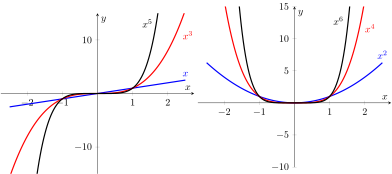
\includegraphics[width=0.9\columnwidth]{figures/0-6-fig2.pdf}
	\end{center}     
\caption{Positive odd powers of $x$ (left) and positive even powers of $x$ (right)}     
\label{F:0.6.Ex1} 
\end{figure}

For odd values of $n$, the graphs of $x^{n}$ are always increasing.  For even values of
$n$, the graphs of $x^{n}$ decrease until $x=0$ and then increase afterwards. See Figure
\ref{F:0.6.Ex1} for several examples of power functions. We can classify the {\it end
behavior} of the graphs by describing what happens as $x\to\infty$ and as $x\to-\infty$.
For odd $n$, $x^{n}\to -\infty$ as $x\to-\infty$ and $x^{n}\to\infty$ as $x\to\infty$.
Graphs of odd power functions go in opposite directions on the left and right.  For even
$n$, $x^{n}\to \infty$ as $x\to-\infty$ and $x^{n}\to\infty$ as $x\to\infty$.  Graphs of
even power functions go in the same direction on the left and right.

\begin{activity}\label{A:0.6.1}
Power functions and exponential functions appear somewhat similar in their formulas, but behave differently in many ways.  
\ba
	\item Compare the functions $f(x)=x^2$ and $g(x)=2^x$ by graphing both functions in several viewing windows.  Find the points of intersection of the graphs.  Which function grows more rapidly when $x$ is large?
    \item Compare the functions $f(x)=x^{10}$ and $g(x)=2^x$ by graphing both functions in several viewing windows.  Find the points of intersection of the graphs.  Which function grows more rapidly when $x$ is large?
	\item Make a conjecture: As $x\to\infty$, which dominates, $x^n$ or $a^x$ for $a>1$?
% 	\item Suppose you are offered a job that lasts one month.  You have the option of being paid in one of two ways: (1) One million dollars at the end of the month; or (2) One cent on the first day of the month, two cents on the second day, four cents on the third day, and, in general, $2^{n-1}$ cents on the $n^{th}$ day.  Which option should you choose?
% 	\item How much different (shorter or longer) would the work period need to be for your answer to the previous question change?
        \ea

\end{activity}
\begin{smallhint}
You may need to use a graphing tool for this activity.
\end{smallhint}
\begin{bighint}
You may need to use a graphing tool for this activity. To see the full behavior of the
functions you will need to use the zoom and pan tools on your graphing technology.
\end{bighint}
\begin{activitySolution}
   \ba
        \item The functions $f(x) = x^2$ and $g(x) = 2^x$ intersect at three points:
            $(-0.77,0.59)$, $(2,4)$, and $(4,16)$.  After the point $(4,16)$ the
            exponential function $g(x) = 2^x$ grows more rapidly.
        \item The functions $f(x) = x^{10}$ and $g(x) = 2^x$ intersect at three points:
            $(-0.94, 0.52)$, $(1.08, 2.11)$, and another point near $x \approx 60$.  The
            $y$ values on both functions at the third point are very very large, but at
            this point the function $g(x) = 2^x$ dominates the power function $f(x) =
            x^{10}$.
        \item For $a>1$ the exponential function will always dominate the power function.
        \item 
   \ea
\end{activitySolution}

\aftera


\subsection*{Polynomial Functions} 

\begin{definition}[polynomial functions]
A polynomial function is a function of the form
	\[
		p(x)=a_{n}x^{n} + a_{n-1}x^{n-1}+\cdots + a_{1}x + a_{0}
	\]
where $n$ is a nonnegative integer and $a_{n}\ne 0$.  Here $n$ is the {\it degree} of the
polynomial, and $a_{n}$, $a_{n-1}$, \ldots, $a_{1}$, $a_{0}$ are the {\it coefficients}.
\end{definition}

When we study the graphs of functions, there are several common features we're interested in.  
\begin{itemize}
	\item How does the graph behave as $x\to\infty$ and as $x\to-\infty$? (Does it grow without bound? Does it level off? Does it oscillate?) 
	\item Where does the graph cross the $x$-axis? How many times? 
	\item Where does the graph change directions? How many times?
\end{itemize}

For many functions, these questions can be difficult to answer and require specialized
mathematics (like Calculus for example).  For polynomials, though, there are some
relatively simple results.  First, the end behavior of a polynomial is determined by its
degree and the sign of the lead coefficient.  Polynomials with even degree behave like
power functions with even degree, and polynomials with odd degree behave like power
functions like odd degree. Figures \ref{F:0.6.PolyEndBehavior} and
\ref{F:0.6.PolyEndBehavior2} demonstrate this for two different fourth degree polynomials.

% \def\scl{0.75}
\begin{figure}[ht!]
	\begin{center}
% 		\begin{tikzpicture}[line cap=round,line join=round,>=triangle 45, x=0.5cm,
%             y=0.006cm, scale=\scl] 
% 			\draw[<->,color=black] (-6,0.0) -- (7,0.0); 
% 			\foreach \x in {-4,-2,2,4,6} 
% 			\draw[shift={(\x,0)},color=black] (0pt,2pt) -- (0pt,-2pt) node[below] {\footnotesize $\x$}; 
% 			\draw[<->,color=black] (0.0,-100) -- (0.0,850); 
% 			\foreach \y in {,800} 
% 			\draw[shift={(0,\y)},color=black] (2pt,0pt) -- (-2pt,0pt) node[left] {\footnotesize $\y$}; 
% 			\draw[color=black] (0pt,-10pt) node[right] {\footnotesize $0$}; 
% 			\clip(-6,-200) rectangle (7,850); 
%             \draw[very thick, blue, smooth,samples=100,domain=-6:7] plot(\x,{(\x)^(4.0)}); 
% 			\begin{scriptsize} 
% 				\draw[color=black] (-0.5,-150) node {$y=x^{4}$}; 
% 			\end{scriptsize} 
% 		\end{tikzpicture}   
% 		\begin{tikzpicture}[line cap=round,line join=round,>=triangle 45, x=0.5cm, y=0.006cm, scale=\scl] 
% 			\draw[<->,color=black] (-6,0.0) -- (7,0.0); 
% 			\foreach \x in {-4,-2,2,4,6} 
% 			\draw[shift={(\x,0)},color=black] (0pt,2pt) -- (0pt,-2pt) node[below] {\footnotesize $\x$}; 
% 			\draw[<->,color=black] (0.0,-100) -- (0.0,850); 
% 			\foreach \y in {,800} 
% 			\draw[shift={(0,\y)},color=black] (2pt,0pt) -- (-2pt,0pt) node[left] {\footnotesize $\y$}; 
% 			\draw[color=black] (0pt,-10pt) node[right] {\footnotesize $0$}; 
% 			\clip(-6,-200) rectangle (7,850); 
% 			\draw[very thick, blue, smooth,samples=100,domain=-6:7] plot(\x,{(\x)^(4.0)-2.0*(\x)^(3.0)-12.0*(\x)^(2.0)+3.0*(\x)-4.0}); 
% 			\begin{scriptsize} 
% 				\draw[color=black] (-0.5,-150) node {$y=x^{4} - 2x^{3} - 12x^{2} + 3x - 4$}; 
% 			\end{scriptsize} 
% 		\end{tikzpicture}
        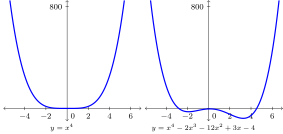
\includegraphics[width=0.8\columnwidth]{figures/0-6-fig3.pdf}
	\end{center}      
\caption{Local behavior of two fourth-degree polynomials.  At this level, we can clearly see the differences between these two functions.}
\label{F:0.6.PolyEndBehavior}
\end{figure}

\begin{figure}[ht!]
	\begin{center}
% 		\begin{tikzpicture}[line cap=round,line join=round,>=triangle 45, x=1.5cm, y=0.35cm, scale=\scl] 
% 			\draw[<->,color=black] (-2,0.0) -- (2,0.0); 
% 			\foreach \x in {-20,-10,10,20} 
% 			\draw[shift={(\x/10,0)},color=black] (0pt,2pt) -- (0pt,-2pt) node[below] {\footnotesize $\x$}; 
% 			\draw[->,color=black] (0.0,-2) -- (0.0,15); 
% 			\draw[shift={(0,14)},color=black] (2pt,0pt) -- (-2pt,0pt) node[left] {\footnotesize $160,000$}; 
% 			\draw[color=black] (0pt,-10pt) node[right] {\footnotesize $0$}; 
% 			\clip(-2,-4) rectangle (2,15); 
% 			\draw[very thick, blue, smooth,samples=100,domain=-2:2] plot(\x,{(\x)^(4.0)}); 
% 			\begin{scriptsize} 
% 				\draw[color=black] (-0.5,-3) node {$y=x^{4}$}; 
% 			\end{scriptsize} 
% 		\end{tikzpicture}  
% 		\begin{tikzpicture}[line cap=round,line join=round,>=triangle 45, x=1.5cm, y=0.35cm, scale=\scl] 
% 			\draw[<->,color=black] (-2,0.0) -- (2,0.0); 
% 			\foreach \x in {-20,-10,10,20} 
% 			\draw[shift={(\x/10,0)},color=black] (0pt,2pt) -- (0pt,-2pt) node[below] {\footnotesize $\x$}; 
% 			\draw[->,color=black] (0.0,-2) -- (0.0,15); 
% 			\draw[shift={(0,14)},color=black] (2pt,0pt) -- (-2pt,0pt) node[left] {\footnotesize $160,000$}; 
% 			\draw[color=black] (0pt,-10pt) node[right] {\footnotesize $0$}; 
% 			\clip(-2,-4) rectangle (2,15); 
% 			\draw[very thick, blue, smooth,samples=100,domain=-2:2] plot(\x,{(\x)^(4.0)}); 
% 			\begin{scriptsize} 
% 				\draw[color=black] (-0.5,-3) node {$y=x^{4} - 2x^{3} - 12x^{2} + 3x - 4$}; 
% 			\end{scriptsize} 
% 		\end{tikzpicture}  
        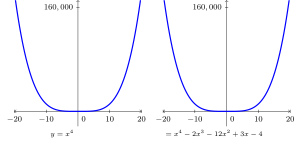
\includegraphics[width=0.8\columnwidth]{figures/0-6-fig4.pdf}
	\end{center}      
\caption{Long-term behavior of two fourth-degree polynomials.  At this scale, the two functions are nearly indistinguishable.}
\label{F:0.6.PolyEndBehavior2}
\end{figure}

\begin{theorem}
%Roots of polynomials
	A polynomial of degree $n$ has at most $n$ real zeros and at most $n-1$ turning points.\label{T:0.6.1}
\end{theorem}

\begin{theorem}\label{T:0.6.2}
%Polynomial roots and factors
	Let $p(x)$ be a polynomial.  If $x = a$ is a zero of $p$ (i.e. $p(a)=0$), then $(x-a)$ is a factor of $p$.
\end{theorem}

Theorems \ref{T:0.6.1} and \ref{T:0.6.2} are each fairly simple to state but very powerful.  Theorem \ref{T:0.6.1} gives us a quick way to determine the degree of a polynomial from its graph and is frequently used to determine how many solutions to expect from certain types of equations.  
Theorem \ref{T:0.6.2} provides us with a way to construct polynomials that pass through specific points.  

\begin{activity}\label{A:0.6.2}
	For each of the following graphs, find a possible formula for the polynomial of lowest degree that fits the graph.
    \def\scl{0.7}
				\begin{center}
%                     \begin{tikzpicture}[scale=\scl]
%                         \begin{axis}[axis lines=center, xmin=-4, xmax=2, ymin=-5, ymax=2,
%                             title={Plot (a)}]
%                             \addplot[very thick, blue, smooth,samples=100,domain=-4.0:2.0] {((x)-1.0)*((x)+3.0)};
%                         \end{axis}
%                     \end{tikzpicture}
%                     \begin{tikzpicture}[scale=\scl]
%                         \begin{axis}[axis lines=center, xmin=-3, xmax=3.5, ymin=-8.5, ymax=6,
%                             title={Plot (b)}, ytick={-8,-6,-4,-2,2,4,6}]
%                             \addplot[very thick, blue, smooth,samples=100,domain=-3:3.5] {0-((x)+2.0)*((x)-3.0)*((x)-1.0)};
%                         \end{axis}
%                     \end{tikzpicture}
%                     \begin{tikzpicture}[scale=\scl]
%                         \begin{axis}[axis lines=center, xmin=-2, xmax=3, ymin=-3, ymax=2,
%                             title={Plot (c)}]
%                             \addplot[very thick, blue, smooth,samples=100,domain=-2:3] {((x)+1.0)*((x)-2.0)*((x)-1.0)*((x)-1.0)};
%                         \end{axis}
%                     \end{tikzpicture}
% % 					\begin{tikzpicture}[line cap=round,line join=round,>=triangle 45, x=1.0cm, y=0.86cm] 
% % 						\draw[->,color=black] (-4.0,0.0) -- (2.0,0.0);
% % 						\foreach \x in {-4,-3,-2,-1,1}
% % 						\draw[shift={(\x,0)},color=black] (0pt,2pt) -- (0pt,-2pt) node[below] {\footnotesize $\x$};
% % 						\draw[->,color=black] (0.0,-5.0) -- (0.0,2.0);
% % 						\foreach \y in {-5,-4,-3,-2,-1,1}
% % 						\draw[shift={(0,\y)},color=black] (2pt,0pt) -- (-2pt,0pt) node[left] {\footnotesize $\y$};
% % 						\draw[color=black] (0pt,-10pt) node[right] {\footnotesize $0$};
% % 						\clip(-4.0,-5.0) rectangle (2.0,2.0);
% % 						\draw[very thick, blue, smooth,samples=100,domain=-4.0:2.0] plot(\x,{((\x)-1.0)*((\x)+3.0)});
% % 					\end{tikzpicture}   
% % 					\begin{tikzpicture}[line cap=round,line join=round,>=triangle 45, x=0.86cm, y=0.33cm] 
% % 						\draw[<->,color=black] (-3.5,0.0) -- (3.5,0.0); 
% % 						\foreach \x in {-3,-2,-1,1,2,3} 
% % 						\draw[shift={(\x,0)},color=black] (0pt,2pt) -- (0pt,-2pt) node[below] {\footnotesize $\x$}; 
% % 						\draw[->,color=black] (0.0,-10) -- (0.0,8); 
% % 						\foreach \y in {-8,-6,-4,-2,2,4,6}
% % 						\draw[shift={(0,\y)},color=black] (2pt,0pt) -- (-2pt,0pt) node[left] {\footnotesize $\y$}; 
% % 						\draw[color=black] (0pt,-10pt) node[right] {\footnotesize $0$}; 
% % 						\clip(-3.5,-10) rectangle (3.5,8); 
% % 						\draw[very thick, blue, smooth,samples=100,domain=-3.5:3.5] plot(\x,{0-((\x)+2.0)*((\x)-3.0)*((\x)-1.0)});
% % 					\end{tikzpicture}   
% % 					\begin{tikzpicture}[line cap=round,line join=round,>=triangle 45, x=1.2cm, y=1.1cm] 
% % 						\draw[<->,color=black] (-2,0.0) -- (3,0.0); 
% % 						\foreach \x in {-2,-1,1,2,3} 
% % 						\draw[shift={(\x,0)},color=black] (0pt,2pt) -- (0pt,-2pt) node[below] {\footnotesize $\x$}; 
% % 						\draw[->,color=black] (0.0,-3.5) -- (0.0,2); 
% % 						\foreach \y in {-3,-2,-1,1,2}
% % 						\draw[shift={(0,\y)},color=black] (2pt,0pt) -- (-2pt,0pt) node[left] {\footnotesize $\y$}; 
% % 						\draw[color=black] (0pt,-10pt) node[right] {\footnotesize $0$}; 
% % 						\clip(-2,-3.5) rectangle (3,2); 
% % 						\draw[very thick, blue, smooth,samples=100,domain=-2:3] plot(\x,{((\x)+1.0)*((\x)-2.0)*((\x)-1.0)*((\x)-1.0)}); 
% % 					\end{tikzpicture}   
                    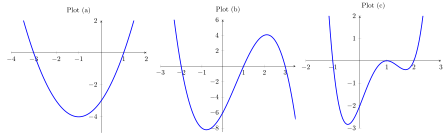
\includegraphics[width=0.99\columnwidth]{figures/0-6-fig5.pdf}
				\end{center}      
\end{activity}
\begin{smallhint}
How many roots are there and how do the ends behave?
\end{smallhint}
\begin{bighint}
    You may want to use Theorems \ref{T:0.6.1} and \ref{T:0.6.2} to determine the degree
    of the polynomial as well as the roots and factors.
\end{bighint}
\begin{activitySolution}
   \ba
        \item This function clearly has two roots and the ends show the same behavior.
            This indicates that this is likely a degree 2 polynomial (a quadratic).  Based
            on the roots $x=-2$ and $x=1$ the factors are $(x+2)$ and $(x-1)$ so the
            polynomial is of the form $a(x) = C(x+2)(x-1)$.  Finally, it appears that the
            point $(-1,-4)$ is on the curve so $C=2$ and the polynomial is 
            \[ a(x) = 2(x+2)(x-1). \]
        \item This function clearly has three roots and the ends show the opposite
            behavior.  Since the right-hand side of the function tends down we expect a
            negative leading coefficient.  Based on the roots $x=-2$, $x=1$, and $x=3$ the
            factors are $(x+2)$, $(x-1)$, and $(x-3)$ and the polynomial takes the form
            $b(x) = C(x+2)(x-1)(x-3)$.  The point $(-1,-8)$ appears to be on the graph so
            $C = -1$ and the polynomial is
            \[ b(x) = -(x+2)(x-1)(x-3). \]
        \item This function clearly has three roots but the end behavior indicates an even
            degree polynomial.  The root at $x=1$ is special since we do not cross the $x$
            axis.  Hence, the factors are $(x+1)$, $(x-1)$, $(x-1)$, and $(x-2)$.  Notice
            that the $(x-1)$ root is listed twice, and hence the polynomial takes the form
            $c(x) = C(x+1)(x-1)^2(x-2)$.  The point $(0,-2)$ appears to be on the graph so
            $C = 1$ and the polynomial is
            \[ c(x) = (x+1)(x-1)^2(x-2). \]
   \ea
\end{activitySolution}

\aftera


\subsection*{Rational Functions}

\begin{definition}[rational functions]
	A rational function is a ratio of two polynomial functions
		\[ 
			f(x) = P(x)/Q(x)
		\]
	where $P$ and $Q$ are polynomials.  The domain is the set of all real numbers for which $Q(x)\ne 0$
\end{definition}

\begin{definition}[horizontal asymptotes]
	A function $f$ has a horizontal asymptote $y = a$ if the distance between the $f$ and the line $y=a$ becomes arbitrarily small when $x$ becomes sufficiently large.
	Alternatively, a horizontal asymptote is a line that a function approaches as $x \to \infty$ or as $x \to -\infty$. 
\end{definition}

\begin{definition}[vertical asymptotes]
    A function $f$ has a vertical asymptote at a point $x = b$ if the function becomes arbitrarily large as $x \to b$.
\end{definition}

The graphs of rational functions may have vertical asymptotes only where the denominator is zero.  However, there are many examples of rational functions that do not have a vertical asymptote even at a point where the denominator is zero. (For instance, try graphing the function $f(x)=\displaystyle{\frac{x^{2}-1}{x-1}}$).

\begin{activity}\label{A:0.6.3}
% The purpose of this activity is to prompt students to start thinking about vertical asymptotes (and division by 0) in terms of limits.  
\ba
		\item Suppose $f(x) = x^{2}+ 3x + 2$ and $g(x) = x - 3$.  
			\begin{enumerate}
                \item[(i)] What is the behavior of the function $h(x) = \displaystyle{\frac {f(x)}{g(x)}}$ near $x = -1$? (i.e. what happens to $h(x)$ as $x\to -1$?) near $x = -2$? near $x = 3$?
                \item[(ii)] What is the behavior of the function $k(x) = \displaystyle{\frac {g(x)}{f(x)}}$ near $x = -1$? near $x = -2$? near $x = 3$?
			\end{enumerate}
		\item Suppose $f(x) = x^{2} - 9$ and $g(x) = x - 3$.  
			\begin{enumerate}
                \item[(i)] What is the behavior of the function $h(x) = \displaystyle{\frac {f(x)}{g(x)}}$ near $x = -3$? (i.e. what happens to $h(x)$ as $x\to -3$?) near $x = 3$?
                \item[(ii)] What is the behavior of the function $k(x) = \displaystyle{\frac {g(x)}{f(x)}}$ near $x = -3$? near $x = 3$?
			\end{enumerate}
% 		\item Suppose $f(x) = \sin{x}$ and $g(x) = x$.
% 			\begin{enumerate}
%                 \item[(i)] What is $f(0)$? What is $g(0)$?
%                 \item[(ii)] What is the behavior of the function $h(x) = \displaystyle{\frac {f(x)}{g(x)}}$ near $x = 0$? (i.e. what happens to $h(x)$ as $x\to 0$?)
%                 \item[(iii)] What is the behavior of the function $k(x) = \displaystyle{\frac {g(x)}{f(x)}}$ near $x = 0$?
% 			\end{enumerate}
\ea

\end{activity}
\begin{smallhint}
    Watch carefully for division by zero.  That is where a vertical asymptote is possible.
\end{smallhint}
\begin{bighint}
    Watch carefully for division by zero.  That is where a vertical asymptote is possible.
\end{bighint}
\begin{activitySolution}
   \ba
        \item For $f(x) = x^2+3x+2$ and $g(x) = x-3$ when we form the function $h(x) =
            f(x)/g(x)$ we get $h(x) = \frac{x^2+3x+2}{x-3}$.  Notice that $h(-1) = 0$ and
            $h(-2) = 0$ since $f(-1) = f(-2) = 0$ and $g(-2) \neq 0$.  At $x=3$, on the
            other hand, $g(x) = 0$ and there is a vertical asymptote on the function
            $h(x)$.

            For $k(x) = g(x) / f(x)$.  The vertical asymptotes occur at $x=-2$ and $x=-1$
            and a zero occurs at $x=3$.
        \item For $f(x) = x^2-9$ and $g(x) = x-3$ we see immediately that $f(x)$ can be
            factored to $f(x) = (x-3)(x+3)$ and hence the function $h(x) = f(x)/g(x)$
            simplifies to $h(x) = x+3$ when $x$ is not $3$.  When $x=3$ there is a
            discontinuity in the graph but this is not a vertical asymptote since the
            discontinuity can be removed algebraically.

            For $k(x) = g(x)/f(x)$ we simplify to $k(x) = 1/(x+3)$ when $x$ is not $3$.
            Therefore there is a vertical asymptote at $x=-3$ and a removable
            discontinuity at $x=3$.
   \ea
\end{activitySolution}

\aftera
  % Vertical Asymptotes and 0/0

\begin{activity}\label{A:0.6.4}

%The purpose of this activity is to encourage students to think of horizontal asymptotes in terms of "dominance" of the numerator over denominator (or vice versa).  
	
\ba
		\item Suppose $f(x) = x^{3} + 2x^{2}-x + 7$ and $g(x) = x^{2} + 4x + 2$.  
			\begin{enumerate}
				\item Which function dominates as $x \to \infty$?
				\item What is the behavior of the function $h(x) = \displaystyle{\frac {f(x)}{g(x)}}$ as $x \to \infty$?
				\item What is the behavior of the function $h(x) = \displaystyle{\frac {g(x)}{f(x)}}$ as $x \to \infty$?
			\end{enumerate}
		\item Suppose $f(x) = 2x^{4} - 5x^{3} + 8x^{2} - 3x - 1$ and $g(x) = 3x^{4} - 2x^{2} + 1$
			\begin{enumerate}
				\item Which function dominates as $x \to \infty$?
				\item What is the behavior of the function $h(x) = \displaystyle{\frac {f(x)}{g(x)}}$ as $x \to \infty$?
				\item What is the behavior of the function $h(x) = \displaystyle{\frac {g(x)}{f(x)}}$ as $x \to \infty$?
			\end{enumerate}
        \item Suppose $f(x) = e^{x}$ and $g(x) = x^{10}$.
			\begin{enumerate}
				\item Which function dominates as $x \to \infty$ as $x \to \infty$?
				\item What is the behavior of the function $h(x) = \displaystyle{\frac {f(x)}{g(x)}}$ as $x \to \infty$?
				\item What is the behavior of the function $h(x) = \displaystyle{\frac {g(x)}{f(x)}}$ as $x \to \infty$?
			\end{enumerate}
\ea

\end{activity}\aftera
  % Horizontal Asymptotes and infinity/infinity.

\begin{activity}\label{A:0.6.5}
	For each of the following functions, determine (1) whether the function has a horizontal asymptote, and (2) whether the function crosses its horizontal asymptote.
\ba
		\item $f(x)=\displaystyle{\frac {x+3}{5x-2}}$
		\item $g(x)=\displaystyle{\frac {x^{2}+2x-1}{x-1}}$
		\item $h(x)=\displaystyle{\frac {x+1}{x^{2}+2x-1}}$
\ea
\end{activity}
\begin{smallhint}
    A horizontal asymptote occurs where the function approaches a value  as $x\to\infty$.
    It is possible for a function to cross a horizontal asymptote.
\end{smallhint}
\begin{bighint}
    A horizontal asymptote occurs where the function approaches a value  as $x\to\infty$.
    It is possible for a function to cross a horizontal asymptote.
\end{bighint}
\begin{activitySolution}
   \ba
        \item For $f(x) = \frac{x+3}{5x-2}$ the degrees of the two polynomials are both $1$
            so the numerator and denominator grow at the same rate.  The horizontal
            asymptote will be the ratio of the coefficients: $f(x) \to
            \frac{1}{5}$ as $x \to \infty$.  The graph does not cross the horizontal
            asymptote.
        \item In this case where $g(x) = \frac{x^2+2x-1}{x-1}$ the degree of the numerator
            is larger than the degree of the denominator so $g(x) \to \infty$ as
            $x\to\infty$ and there is no horizontal asymptote.
        \item In this case where $h(x) = \frac{x+1}{x^2+2x-1}$ the degree of the
            denominator is larger than the degree of the numerator so $h(x) \to 0$ as $x
            \to \infty$.  Therefore, there is a horizontal asymptote at $y=0$.  Observe
            that $h(-1) = 0$ so the function's graph does indeed cross the horizontal
            asymptote.
   \ea
\end{activitySolution}

\aftera
  % Crossing Horizontal Asymptotes



\begin{summary}
	\item A polynomial of degree $n$ has at most $n$ real zeros and $n-1$ turning points.
	\item The degree of a polynomial function determines the end behavior of its graph.  If the degree of a polynomial is even, then the end behavior is the same in both directions.  If the degree of a polynomial is odd, then the end behavior on the left is the opposite of the behavior on the right.
	\item A rational function is a function of the form $f(x)=\frac{P(x)}{Q(x)}$, where $P(x)$ and $Q(x)$ are both polynomials.
	\item A rational function $f(x)=\frac{P(x)}{Q(x)}$ may have a vertical asymptote whenever $Q(x)=0$.
	\item The end behavior of the graph of a rational function is determined by the degrees of the polynomials in the numerator and denominator. (See Activity \ref{A:0.6.4}).
\end{summary}

% exercises go here
\begin{exercises} 

\item Without the aid of a graphing tool match the polynomials to its corresponding graph.
    \begin{flalign*}
        f(x) &= x^3 + 3x^2 - 4x - 12 \\
        g(x) &= -\frac{1}{4}(x-1)^3(x+3) \\
        h(x) &= \frac{1}{3}x^3(x+2)(x-3)^2 \\
        k(x) &= -2x^3-x^2+x
    \end{flalign*}
    \begin{center}
        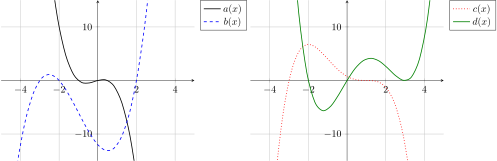
\includegraphics[width=0.99\columnwidth]{figures/0-6-fig6.pdf}
    \end{center}
\begin{exerciseSolution}
\end{exerciseSolution}


\item The cost in dollars for removing $p$ percent of pollutants from a river is 
    \[ C(p) = \frac{61700p}{100-p}. \]
    \ba
        \item Find the cost for removing 20\%.
        \item Find the cost for removing half of the pollutants.
        \item What is the smallest value $p$ can be?
        \item What is the largest value $p$ can be?
        \item What is the value of $C(p)$ as $p \to 100$?  What is the meaning of this in
            the context of the problem?
    \ea
\begin{exerciseSolution}
\end{exerciseSolution}

\item For the function 
    \[ f(x) = \frac{2x-6}{(-6x-1)(6x-6)}, \]
    \ba
        \item what are the vertical asymptotes?
        \item what are the horizontal asymptotes?
        \item what are the coordinates of the $x$ intercepts?
    \ea
\begin{exerciseSolution}
\end{exerciseSolution}

\item Square cuts of the same size are cut from a flat rectangular piece of cardboard. The
    remaining cardboard is folded into a lidless box. Assume that the cardboard originally
    measures 20 inches by 12 inches. Let $x$ be the length of one side of the square cut (at
    this point you should stop and draw a picture).
    \ba
        \item Write a function describing the volume of the resulting box in terms of $x$.
        \item What is an appropriate domain for the volume function?  Plot the volume function
            over the domain.
        \item Write a function describing the surface area of the box in terms of $x$.
        \item Is the domain different for the surface area function?  Why / why not?  Plot
            the surface area function over its appropriate domain.
    \ea

\end{exercises}
\afterexercises


\clearpage
